% !TEX root = ../../Rapport/rapport.tex
\section{Sur le problème de la couverture sommet minimale}

\subsection{Première approche : la programmation linéaire en nombres entiers}

\subsubsection{(a) Justification de l'utilisation de la Programmation Linéaire en Nombres Entiers}

On considère le problème de la couverture minimale sous la forme suivante : $$
\left \lbrace \begin{array}{l}
	\min z = \sum\limits_{j=1}^n x_j\\
	x_r + x_s \geq 1, \quad \forall \{v_r, v_s\} \in E \\
	x_j \in \{0,1\} \quad j = 1, \ldots, n
\end{array} \right .
$$

La fonction objectif représente le nombre de sommets utilisés par la solution du problème. Le fait
de minimiser la fonction objectif permet d'assurer la couverture minimale. Chacune des clauses est
relative à une arête du graphe, et impose qu'au moins un des sommets adjacents à cette arête soit
dans la couverture.

On a donc bien un problème de Programmation Linéaire en Nombres Entiers permettant de résoudre le problème de la couverture minimale.

\subsubsection{(b) Justification des clauses}

Considérons le graphe donné par la figure \ref{triangle}. 

\begin{figure}
	\begin{center}
		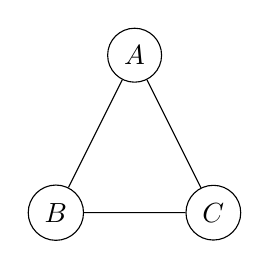
\begin{tikzpicture}
			\tikzset{node/.style={circle, draw=black}};
			\node[node] (A) at (0,2) {$A$};
			\node[node] (B) at (-1, 0) {$B$};
			\node[node] (C) at (1, 0) {$C$};

			\draw (A) -- (B) -- (C) -- (A);
		\end{tikzpicture}
	\end{center}
	\label{triangle}
	\caption{Exemple}
\end{figure}

Sur ce graphe, le programme linéaire en nombres entiers est le suivant :$$
\left \{ \begin{array}{l}
		\min z = x_A + x_B + x_C\\
		x_A + x_B \geq 1 \\
		x_A + x_C \geq 1 \\
		x_B + x_C \geq 1 \\
		x_A, x_B, x_C \in \{0, 1\}
	\end{array} \right .
	$$
Il est très simple ici de comprendre pourquoi il est impossible de considérer le programme linéaire
suivant :$$
\left \{ \begin{array}{l}
		\min z = x_A + x_B + x_C\\
		x_A + x_B = 1 \\
		x_A + x_C = 1 \\
		x_B + x_C = 1 \\
		x_A, x_B, x_C \in \{0, 1\}
	\end{array} \right .
	$$

Ce programmme ne permet pas de résoudre la couverture minimale sur le graphe donné par la figure
\ref{triangle}. Quelque soit le sommet choisi dans un premier lieu pour appartenir à la couverture
minimale, il est impossible d'en choisir un second pour compléter cette dernière. Prenons un
exemple, nous forçons le sommet $A$ à appartenir à la couverture minimale (respectivement $B$ et
$C$). Ce choix force : $x_B = 0$ et $x_C = 0$ (respectivement, $x_A = 0$ et $x_C = 0$, et $x_A = 0$
et $x_B$ = 0). Il est donc impossible de respecter la clause $x_B + x_C = 1$, le problème (au vu de
sa modélisation) n'aurait donc pas de solution, or le graphe de la figure \ref{trisol} montre le
contraire.

\begin{figure}
	\begin{center}
		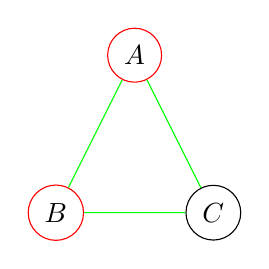
\begin{tikzpicture}
			\tikzset{node/.style={circle, draw=black}};
			\node[node,draw=red] (A) at (0,2) {$A$};
			\node[node,draw=red] (B) at (-1, 0) {$B$};
			\node[node] (C) at (1, 0) {$C$};

			\draw[green] (A) -- (B) -- (C) -- (A);
		\end{tikzpicture}
	\end{center}
	\label{trisol}
	\caption{Solution}
\end{figure}

\subsubsection{(c) Une borne inférieure des solutions optimales}

On cherche à montrer qu'une solution optimale du programme linéaire en nombres entiers est une borne
inférieure de toute solution optimale du programme relaxé. Raisonnons par l'absurde et considérons
une solution optimale du programme linéaire, notée $n^*$ telle qu'il existe $x^*$ solution optimale du problème
relaxé vérifiant $x^* < n^*$. Toute solution du programme linéaire est solution du programme
relaxé\footnote{Une solution appartenant à $\mathbb{N}$ appartient aussi à $\mathbb{R}$}. Ceci
implique : $n^*$ solution du programme relaxé, et donc $x^* < n^*$ impossible. On a donc : $n^* \leq
x^*$ ce qui est la définition d'une borne inférieure.

\subsubsection{(d) A propos de la relaxation de contrainte}

Pour démontrer que la relaxation des contraintes d'intégrité implique $x_r \geq \frac{1}{2}$ ou $x_s
\geq \frac{1}{2}$, le raisonnement par l'absurde sera utilisé. 
Soient $x_s$ et $x_r$ les variables relatives aux sommets $r$ et $s$ adjacents à l'arête $(rc)$ et
telles que, après relaxation des contraintes, on a : $x_r < \frac{1}{2}$ \underline{et} $x_s <
\frac{1}{2}$. On en déduit donc que $x_r + x_s < 1$ et donc la contrainte liée à l'arête $(rs)$ est
violée, l'hypothèse de départ est donc fausse. On a donc, $\forall (rs) \in V : x_r \geq \frac{1}{2}
\mbox{ et } x_s \geq{1}{2}$.

\subsubsection{(e) Une 2-approximation}

Mettons en évidence le pire des cas pouvant se présenter : pour une arête $(rs) \in V$, un seul
sommet est nécessaire pour la couverture de cette dernière dans le cas de la couverture minimale,
mais l'algorithme approché retourne : $x_r = x_s = \frac{1}{2}$. Après la phase d'arrondis, on a $x_r
= x_s = 1$ et donc les deux sommets appartiennent à la solution approchée, cette phase multiplie
donc au pire le nombre de sommets (pour chaque clause par 2), ce qui implique que le cardinal de la
solution approximée est au plus 2 fois la solution optimale.

Cet algorithme est donc une 2-approximation.

\subsubsection{(f) Dans le cas d'un graphe valué}
\paragraph{i. Programme linéaire}
$$
\left \lbrace \begin{array}{l}
	\min z = \sum\limits_{(i,j)\in E}{(x_i \times w_{ij} + x_j \times w_{ij})}\\
	x_r + x_s \geq 1, \quad \forall \{v_r, v_s\} \in E \\
	x_j \in \{0,1\} \quad j \in \{1, \ldots, n\}
\end{array} \right .
$$

\paragraph{ii. PLNE avec matrice\\}

Posons la matrice A, la $(n,n)$-matrice d'adjacente du graphe et X le vecteur contenant les variables existentielles définies précédemment. Le PLNE correspondant est le suivant :
$$
\left \lbrace \begin{array}{l}
	\min z = \sum\limits_{(i,j)\in E}{(x_i \times w_{ij} + x_j \times w_{ij})}\\
	A.X \geq 1\\
	x_j \in \{0,1\} \quad j \in \{1, \ldots, n\}
\end{array} \right .
$$

\paragraph{iii. Algorithme 2-approché}
Dans le pire des cas, on prend tous les sommets du graphe et chaque arête est comptée deux fois. La solution optimale admet une borne inférieure égale à la somme du poids des arcs. Donc la valeur de la fonction objectif  dans le pire des cas vaut deux fois la somme totale des poids des arêtes et il existe un algorithme deux-approché (celui qui prend tous les sommets).


\subsection{Seconde approche : la recherche d'un couplage maximal}

\subsubsection{(a) Une 2-approximation}

Commençons par prouver que l'algorithme retourne une couverture des arêtes par les sommets.
Considérons donc une arête $(rs)$ non couverte par l'ensemble de sommets retourné par l'algorithme, par
définition du couplage, il serait donc possible d'ajouter $(rs)$ au couplage. Or le couplage calculé
par l'algorithme est maximal, on en déduit que l'arête $(rs)$ telle qu'elle est définie ne peut
exister et donc que l'ensemble de sommets obtenu couvre l'ensemble des arêtes du graphe.

Appelons $c$ le couplage calculé par l'algorithme et $x^*$ la solution optimale du problème de la
couverture par les sommets, on sait que $\card c \leq \card x^*$, or pour construire la solution
approchée, on ajoute à $C$ les deux extrêmités des arêtes utilisées pour le couplage. On a donc :$$
\card C = 2 \times \card c \leq 2 \times \card x^*$$ $$\Longrightarrow \frac{\card C}{\card x^*} =
2$$

\subsubsection{(b) Exemple de graphe pathologique}

Le graphe suivant met en évidence la borne 2 de l'algorithme.

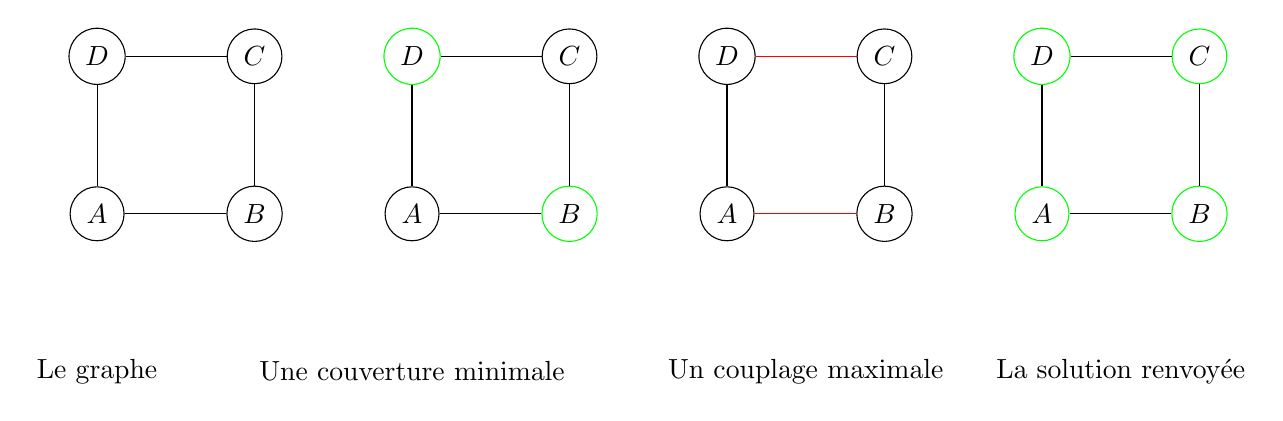
\begin{tikzpicture}
	\tikzset{node/.style={circle}};
	\foreach \x/\xt/\col/\colb/\colc/\cold in {0/A/black/black/black/black,
	4/B/black/green/black/black, 8/C/black/black/red/black, 12/D/green/green/black/black}{
		\node[node, draw=\col] (\xt1) at (\x, 0) {$A$};
		\node[node, draw=\colb] (\xt2) at (\x+2, 0) {$B$};
		\node[node, draw=\col] (\xt3) at (\x+2, 2) {$C$};
		\node[node, draw=\colb] (\xt4) at (\x, 2) {$D$};

		\draw[-, \colc] (\xt1) -- (\xt2);
		\draw[-, \cold] (\xt2) -- (\xt3);
		\draw[-, \colc] (\xt3) -- (\xt4);
		\draw[-, \cold] (\xt4) -- (\xt1);
	}
	\node at (0, -2) {Le graphe};
	\node at (4, -2) {Une couverture minimale};
	\node at (9, -2) {Un couplage maximale};
	\node at (13, -2) {La solution renvoyée};
\end{tikzpicture}

\subsubsection{(c) Application de l'algorithme}
L'application de l'algorithme 3 au graphe d'exemple de la figure 1 donne une couverture $C = \{a_i\} \cup \{b_i\}$ alors que la solution optimale est $C = \{b_i\}$. Si le graphe de la figure 1 est bien le pire des cas pour cet algorithme alors c'est un algorithme $1.6$-approché.

